\chapter{Описание предлагаемого подхода для 2D сегментации}

\section{Распространенный подход}

Было проведено множество исследований в области сегментации КТ изображений легких. Одним из основных подходов является двухшаговая модель, где на первом этапе локализуется предполагаемый 3D участок, содержащий опухоль (Volume of Interest, VOI), а на втором этапе производится непосредственная сегментация внутри выбранного участка. Интуитивное объяснение данной модели состоит в том, что пространство, занимаемое опухолью, достаточно мало по сравнению со всем КТ изображением.

\section{Предлагаемый подход}

Однако было предложено использовать другую модель, производящую сегментацию изображения end-to-end. Данная модель показала отличный результат (первое место) в соревновании Data Science Bowl 2018. В последствии модель была применена к другой задаче - сегментации глиальных опухолей головного мозга по данным МРТ, где показала хороший результат.

Архитектура модели включает очень глубокую encoder-decoder сверточную сеть типа Unet. Также модель использует комбинированную функцию потерь, состоящую из кросс-энтропии наряду с мягкой функцией потерь Дайса. Ожидалось, что модель способна показать хороший результат и в задаче сегментации КТ легких.

На рисунке \ref{mri-sample} визуализирована работа сети на изображении МРТ.

\begin{figure}[!h]
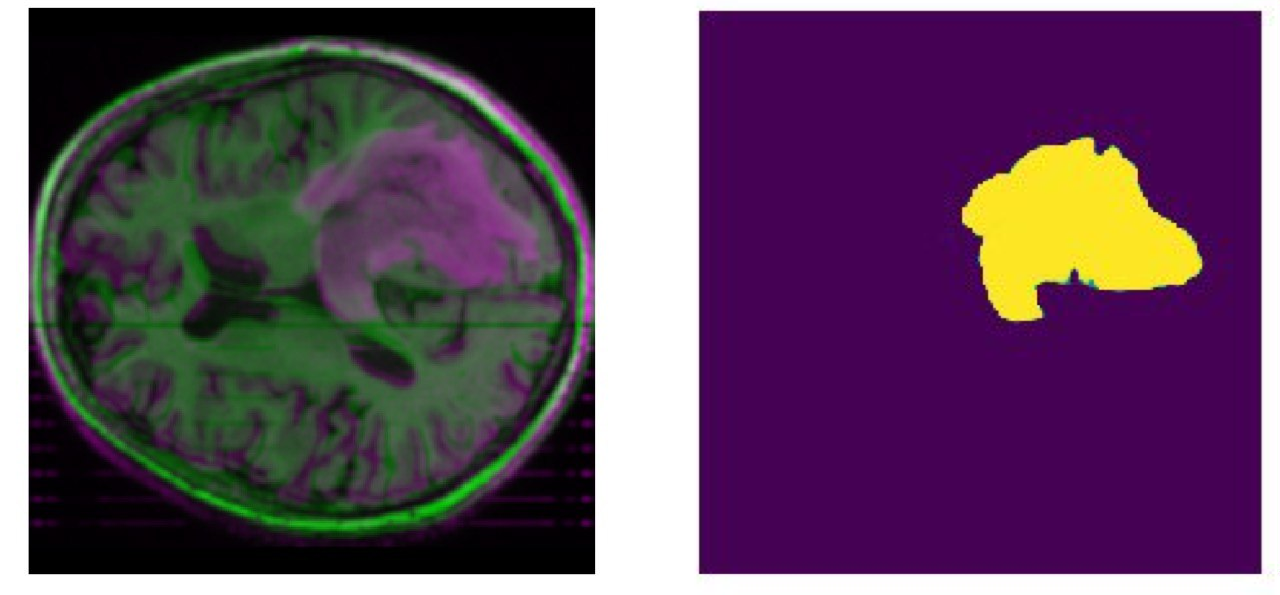
\includegraphics[width=\linewidth]{mri-sample.png}
\caption{Пример работы сети на изображении МРТ}\label{mri-sample}
\centering
\end{figure}